\documentclass[aps,prb,onecolumn,superscriptaddress,floatfix,longbibliography,10pt]{revtex4-2}
% \documentclass[aps,prb,onecolumn,superscriptaddress,floatfix,longbibliography,10pt]{revtex4-2}

\usepackage[utf8]{inputenc}
\usepackage[spanish]{babel}
\usepackage{graphicx}
\usepackage{amsmath}
\usepackage{subcaption}
\usepackage{wrapfig} 
\usepackage[export]{adjustbox}

\usepackage{amsmath,amssymb} % math symbols
\usepackage{bm} % bold math font
\usepackage{graphicx} % for figures
\usepackage{comment} % allows block comments
\usepackage{textcomp} % This package is just to give the text quote '
%\usepackage{ulem} % allows strikeout text, e.g. \sout{text}

\usepackage[spanish]{babel}
% By dafault, spanish changes to a comma as decimal separator; to change to a dot, you can use \decimalpoint:
\decimalpoint

\usepackage{enumitem}
\setlist{noitemsep,leftmargin=*,topsep=0pt,parsep=0pt}

\usepackage{xcolor} % \textcolor{red}{text} will be red for notes
\definecolor{lightgray}{gray}{0.6}
\definecolor{medgray}{gray}{0.4}

%Para las tablas
\usepackage{multirow}

\usepackage{hyperref}
\hypersetup{
colorlinks=true,
urlcolor= blue,
citecolor=blue,
linkcolor= blue,
bookmarks=true,
bookmarksopen=false,
}

% Code to add paragraph numbers and titles
\newif\ifptitle
\newif\ifpnumber
\newcounter{para}
\newcommand\ptitle[1]{\par\refstepcounter{para}
{\ifpnumber{\noindent\textcolor{lightgray}{\textbf{\thepara}}\indent}\fi}
{\ifptitle{\textbf{[{#1}]}}\fi}}
\ptitletrue  % comment this line to hide paragraph titles
\pnumbertrue  % comment this line to hide paragraph numbers

% minimum font size for figures
\newcommand{\minfont}{6}

% Uncomment this line if you prefer your vectors to appear as bold letters.
% By default they will appear with arrows over them.
% \renewcommand{\vec}[1]{\bm{#1}}

%Cambiar Cuadros por Tablas y lista de...
%\renewcommand{\listtablename}{Índice de tablas}
\renewcommand{\tablename}{Tabla}
\renewcommand{\date}{Fecha}

%Para importar imágenes desde una carpeta:
\graphicspath{ {C:/Users/lupam/OneDrive/Escritorio/GitHub/Vapor_en_burbuja_inicial_python/Tesis_informe/Figures}}

\usepackage[bottom]{footmisc} %para que las notas al pie aparezcan en la misma página

\begin{comment}

%Comandos de interés:

* Para ordenar el documento:
\section{Introducción}
\section{\label{sec:Formatting}Formatting} %label para luego hacer referencia a esa sección

\ptitle{Start writing while you experiment} %pone nombre y título al documento dependiendo de si en el header están los comandos \ptitletrue y \pnumbertrue

* Ecuaciones:
\begin{equation}
a^2+b^2=c^2 \,.
\label{eqn:Pythagoras}
\end{equation}

* Conjunto de ecuaciones:
\begin{eqnarray}
\label{eqn:diagonal}
\nonumber d & = & \sqrt{a^2 + b^2 + c^2} \\
& = & \sqrt{3^2+4^2+12^2} = 13
\end{eqnarray}

* Para hacer items / enumerar:
\begin{enumerate}
  \item
\end{enumerate}

\begin{itemize}
  \item
\end{itemize}

* Figuras:
\begin{figure}[h]
    \includegraphics[clip=true,width=\columnwidth]{pixel-compare}
    \caption{}
     \label{fig:pixels}
\end{figure}

* Conjunto de figuras:
(no recuerdo)


* Para hacer referencias a fórmulas, tablas, secciones, ... dentro del documento:
\ref{tab:spacing}

* Para citar
Elementos de .bib
\cite{WhitesidesAdvMat2004}
url
\url{http://www.mendeley.com/}\\

* Agradecimientos:
\begin{acknowledgments}
We acknowledge advice from Jessie Zhang and Harry Pirie to produce Fig.\ \ref{fig:pixels}.
\end{acknowledgments}

* Apéndice:
\appendix
\section{\label{app:Mendeley}Mendeley}

* Bibliografía:
\bibliography{Hoffman-example-paper}

\end{comment}


\begin{document}

% Allows to rewrite the same title in the supplement
\newcommand{\mytitle}{\textcolor{red}{Cálculos Computacionales en Plasmas Producidos por Cavitación Láser y colapso de burbujas - trabajo realizado hasta 27 de Octubre de 2022}}

\title{\mytitle}

\author{Pablo Chehade \\
    \small \textit{pablo.chehade@ib.edu.ar} \\
    \small \textit{Instituto Balseiro, CNEA-UNCuyo, Bariloche, Argentina, 2022} \\}


\begin{abstract}
  \begin{itemize}
    \item \textcolor{red}{TEST2}
    \item Se estudió numéricamente la expansión de una burbuja de cavitación láser. \textcolor{red}{y la compresión}
    \item La evolución temporal se divide en dos partes, cada una de ellas gobernada por fenómenos físicos distintos.
    \item La primera consta desde la creación de la burbuja hasta la expansión rápida al radio máximo. El fenómeno que creemos ocurre es la interacción del láser con los electrones de burbujas microscópicas (bubston) para dar lugar a una avalancha de electrones impulsora de la expansión (fenómeno electromagnético y fluidodinámico). El fenómeno se debe principalmente a la acción de los electrones y las moléculas ionizadas que rodean exteriormente la burbuja.
    \item La segunda, desde el radio máximo hasta su implosión al radio mínimo. En este momento el efecto de los electrones se diluye y comienzan a preponderar efectos de conducción del calor, cambios en la masa contenida dentro de la esfera debido a reacciones químicas, difusión y condensación/evaporación, entre otros. El fenómeno se debe principalmente a la acción de los iones y moléculas dentro y fuera de la burbuja (fenómeno fluidodinámico, termodinámico y químico).
    \item Se exploraron además distintos métodos numéricos y técnicas de resolución computacionales para resolver este problema complejo que inherentemente es del tipo stiff debido a las diferencias de órdenes de magnitud entre las constantes de tiempo involucradas.
  \end{itemize}


\end{abstract}

\maketitle

\section*{Índice}
\textcolor{red}{Buscar en internet cómo hacer un índice en Latex}

\section*{Introducción}


















\section*{Capítulo I: Evolución hasta el radio máximo}

\ptitle{Resumen del capítulo. En este capítulo se discute el proceso a partir del cual un láser incidente en un medio líquido es capaz de producir una burbuja de cavitación}
\begin{itemize}
  \item El proceso se desarrolla en \textcolor{red}{Referencia al Bunkin}
  \item Se parte de un medio líquido, en nuestro caso agua deuterada, en el cual se asume existen micro burbujas de gas (bubstons) agrupadas en clusters en la zona focal del haz de luz. 
  \item Se asume que dentro de cada bubston hay inicialmente un electrón libre
  \item Bajo estas condiciones, se demuestra en el paper que bajo determinadas condiciones de la burbuja y de la intensidad del haz, se desarrolla una avalancha de electrones
  \item Esta produce una presión eléctrica que expande el bubston hasta que los bubstons del cluster se fusionan entre sí y forman una gran burbuja o "núcleo". 
  \item Este efecto se denomina SOC
  \item Explicar brevemente qué ocurre luego
  \item Las cuentas se hacen en el sistema CGS
  \item Contar que el proceso consta de 3 etapas

\end{itemize}

\ptitle{Situación física inicial}
\begin{itemize}
  \item Resumen: en esta sección se explica la situación física inicial antes de la incidencia del láser.
  \item Se parte de un medio líquido en el que se encuentran clusters de burbujas estables (bubstons) de radio $R_0$.
  \item Explicar cómo calcular R0 y dar el valor aproximada
  \item La estabilidad de los bubstons se basa en la condición $R_0 << l_{em}$. Explicar
  \item Se considera que dentro de la burbuja hay al menos un electrón libre
  \item Definir R0 en algún lado
\end{itemize}



\subsection{Avalancha de electrones dentro de los bubston}

En esta sección se explicará el proceso a través del cual aumenta la cantidad de electrones $N_e$ dentro de cada bubston al incidir un láser. Se parte de la hipótesis de que existe al menos un electrón libre en cada uno de ellos. Además, se asume ocurre rápidamente de modo que su radio se mantiene aproximadamente constante. Se encontrará que el aumento de $N_e$ no es indefinido, sino que se alcanza un valor máximo a partir del cual se mantiene constante. También se hallará una condición sobre la intensidad del haz de luz necesaria para que ocurra la avalancha.

\textcolor{red}{La suposición de que el radio se mantiene constante y el proceso ocurre rápidamente es necesaria para, creo, asegurar que solo ocurren 2 fenómenos que contribuyen a la avalancha. Fabián: referenciá al Bunkin para justificar}

\textcolor{red}{En algún lado hay que agregar que tmb hay que suponer que $\tau >> t_0$. Esto implica que el láser está el suficiente tiempo para que se alcance el valor máximo $N_{e \, max}$}.

\ptitle{La avalancha comienza con un electrón dentro de la burbuja inmerso en el campo electromagnético producido por el láser}

Como se mencionó anteriormente, el proceso comienza con al menos un electrón libre dentro de cada bubston. Al incidir el láser, el electrón interactúa con el campo electromagnético oscilatorio y se acelera. En su movimiento choca con las paredes de la burbuja con una frecuencia $\nu_{e w} = \bar{v_e}/R_0$ donde $\bar{v_e}$ es la velocidad media aritmética de los electrones. En cada choque existe una probabilidad de que ionice alguna molécula de la pared, extrayendo un electrón que contribuye a la avalancha, y una probabilidad de que se quede adherido a alguna de ellas, en decrimento de la avalancha. El primer caso ocurre con frecuencia $\nu_i = \dot{\mathcal{E}_e}/\Delta$ donde $\dot{\mathcal{E}_e}$ es la velocidad media de aumento de la energía cinética del electrón ${\mathcal{E}_e}$ debido al movimiento caótico. Mientras que $\Delta$ es la energía de ionización de una molécula de la pared. Esta puede ser mucho menor que la energía de ionización de una molécula individual del líquido y se estima en $\sim 6$ eV. \textcolor{red}{Bunkin referencia a Grand 1979. El paper ya lo descargué, debería leerlo}. El segundo caso ocurre con frecuencia $\nu_{loss} = (\bar{v}_e/R_0) w_{a,e}$ donde $w_{a,e}$ es la probabilidad de adhesión a la pared. De este modo, el número de electrones en el tiempo se encuentra determinado por la ecuación
\begin{equation}
  \frac{dN_e}{dt} = \nu_i N_e - \nu_{loss} N_e.
  \label{eq:dNedt_1}
\end{equation}


\ptitle{Determinación de la frecuencia de ionización}


A continuación se determinará la relación entre $\nu_i$ y las propiedades del láser. Asumiendo que el efecto del campo eléctrico es mayor al magnético, la velocidad $\dot{\mathcal{E}_e}$ corresponde a la potencia promedio $\langle P \rangle$ entregada por el haz de luz a un electrón. Además, considerando que la amplitud de oscilación del electrón es mucho menor a la longitud de onda del haz, el campo eléctrico $E(t)$ se puede considerar uniforme
\[E(t) = E_0 \sin{(w t)},\]
con $w$ frecuencia del haz y $E_0$ amplitud. En base a esto, la posición del electrón está dada clásicamente por la ley de Newton
\[m \dot{v} = -e E(t) -m \nu_{e w} v\]
donde $m$ es la masa del electrón, $v$ su velocidad, $e$ su carga y el término de fricción $m \nu_{e w} v$ representa las colisiones con la pared. Resolviendo la ecuación diferencial para tiempos largos $t \nu_{e w} >> 1$ se obtiene la velocidad
\[v(t) = \frac{e E_0}{m(\nu_{e w}^2 + w^2)}[w \cos{(t w)} - \nu_{e w} \sin{(t w)}]. \]
En base a esta se puede calcular la potencia promedio entregada al electrón 
\[\langle P \rangle = \langle - e E(t) v(t) \rangle = \nu_{e w}\frac{e^2 E_0^2}{2 m w^2} = \nu_{e w} \frac{I}{c n_{e \, cr}}\]
donde $n_{e \, cr} = mw^2/4 \pi e^2$ es la densidad de electrones crítica e $I = \frac{c}{8 \pi} E_0^2$ es la intensidad del haz, con $c$ velocidad de la luz. De este modo, la frecuencia de ionización se puede expresar como $\nu_i = \frac{\nu_{e w}}{\Delta} \frac{I}{c n_{e \, cr}}$

\ptitle{Determinación del nro de electrones en el tiempo y planteo de la condición límite}

Una vez calculada la frecuencia de ionización, se está en condiciones de determinar la evolución de $N_e(t)$. Reemplazando la expresión anterior en \ref{eq:dNedt_1}, se obtiene
\begin{equation}
  \frac{dN_e}{dt} = \nu_{e w} w_{a,e} \left ( \frac{I}{I_0} - 1 \right ) N_e = \beta N_e,
  \label{eq:dNedt_2}
\end{equation}
donde $I_0 = c n_{e \, cr} \Delta w_{a,e}$ es la intensidad mínima del haz necesaria para que $\beta>0$ y, por lo tanto, se produzca la avalancha de electrones. \textcolor{red}{Vale la pena hacer la cuenta con el láser del laboratorio?}. En caso de producirse, la expresión anterior indica un crecimiento exponencial $N_e(t) = N_e(0) e^{\beta t}$. Sin embargo, esto no puede ocurrir. El análisis anterior vale cuando la densidad media de electrones $\bar{n}_e$ es pequeña y por lo tanto se pueden despreciar las colisiones entre electrones, es decir, el camino libre medio de colisión entre electrones $l_{ee}$ es más grande que el tamaño de la burbuja $R_0$ que se asume que no varía. Cuando esto deja de valer, las colisiones de los electrones con la pared comienzan a disminuir, como así también $\nu_{e w}$ y, por lo tanto, el factor $\beta$ en \ref{eq:dNedt_2}. En la competencia de ambos procesos se llegaría a un equilibrio en el que la cantidad de electrones no aumenta. Para determinar tal número máximo de electrones $N_{e, max}$ es necesario conocer la densidad de electrones dentro del bubston.

\ptitle{Cálculo de la densidad media máxima}

A continuación se calculará la distribución de la densidad de electrones $n_e(r)$ dentro de un bubston. Asumiendo la validez de la distribución de Boltzmann \textcolor{red}{y qué otras hipótesis??. Este problema se conoce como el problema de Debye. Esto se discute en $https://en.wikipedia.org/wiki/Debye_length$} y aplicando la ecuación de Poisson, esta densidad es solución del sistema de ecuaciones diferenciales
\[
\left\{\begin{matrix}
  n_e(r) = n_e(0)e^{e \phi / T_e}, 0 \leq r \leq R_0 \\
  \triangledown^2 \phi = 4 \pi e n_e(r)
\end{matrix}\right.
\]
donde $\phi(r)$ es el potencial producido por la densidad de carga y $T_e$ es la temperatura del gas de electrones. Realizando la aproximación $e^{e \phi / T_e} \approx 1 + e \phi/T_e$
se logra despejar la ecuación diferencial para el potencial
\[\triangledown^2 \phi - \phi/a_e^2 = 4 \pi e n_e(0) \]
donde $a_e = \sqrt{T_e/4\pi e^2 n_e(0)}$ es el \textcolor{red}{electron Debye radius. Es lo mismo que el radio de Debye en un plasma?}. Imponiendo la condición de borde $\phi(0) = 0$ se obtiene la solución
\begin{equation}
  \phi(r) = \frac{T_e}{e} \left ( \frac{\sinh{r/a_e}}{r/a_e} - 1   \right ),
  \label{eq:cap1_phi}
\end{equation}
y la distribución de electrones
\begin{equation}
  n_e(r) = n_e(0) \frac{\sinh{r/a_e}}{r/a_e}
  \label{eq:cap1_ne}
\end{equation}


\ptitle{Cálculo de las ctes de la expresión de la densidad máxima}

\begin{itemize}
  \item A partir de la definición de $a_e$ se obtiene una expresión para $n_e(0)$
  \item Solo falta calcular $a_e$.
  \item Esto se puede hacer a partir de la relación de autoconsistencia
  \item \begin{equation}
          N_e = 4 \pi \int_0^{R_0} r^2 n_e(r) dr = \frac{T_e R_0}{e^2} \frac{(R_0/a_e) \cosh{(R_0/a_e)} - \sinh{(R_0/a_e)}}{R_0/a_e}
          \label{eq:cap1_Ne}
        \end{equation}
  \item $a_e$ es solución de la ecuación anterior para dado $N_e$
  \item \ref{fig:cap1_Ne_vs_x}
  \item En base a lo anterior se puede expresar $n_e(r)$
  \item \ref{fig:cap1_densidad_vs_r_vs_Ne}
  \item Discusión del gráfico
  \item Mostrar que los electrones se juntan en su mayoría en el borde de la burbuja. Esta es una capa límite de tamaño $a_e$
  \item Entonces, la condición límite pasa a ser $l_ee = a_e$.
\end{itemize}

\begin{figure}[h]
  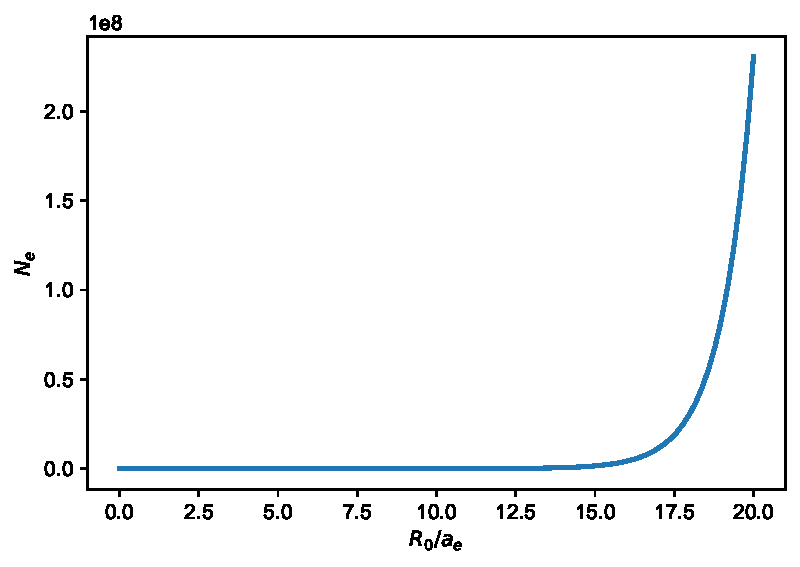
\includegraphics[clip=true,width=\columnwidth]{cap1_Ne_vs_x.pdf}
  \caption{}
    \label{fig:cap1_Ne_vs_x}
\end{figure}

\begin{figure}[h]
  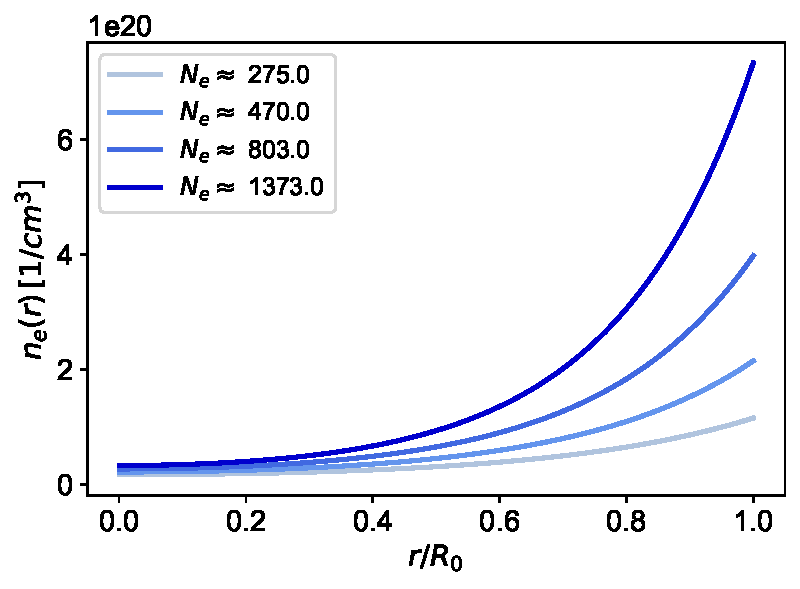
\includegraphics[clip=true,width=\columnwidth]{cap1_densidad_vs_r_vs_Ne.pdf}
  \caption{}
   \label{fig:cap1_densidad_vs_r_vs_Ne}
\end{figure}


\ptitle{Cálculo de $N_{e \, max}$}
\begin{itemize}
  \item $N_e$ alcanza su valor máximo $N_{e \, max}$ en la condición límite $l_{ee} = a_e$.
  \item donde $l_{ee}$ está dado por
  \item expresión con referencia
  \item donde
  \item expresión para $n_e(R_0)$ con label
  \item Para continuar con el desarrollo es necesario introducir la siguiente aproximación.
  \item En base al gráfico de $N_e$ \textcolor{red}{referencia}, para que $N_e$ sea grande, debe ocurrir que $R_0/a_e>>1$.
  \item Bajo este límite se obtiene $N_e \approx \frac{T_e R_0}{2 e^2} e^{R_0/a_e}$
  \item y $n_e(R_0) \approx \frac{T_e}{8 \pi e^2 R_0^2} \frac{R_0}{a_e} e^{R_0/a_e}$
  \item a partir de \ref{eq:cap1_Ne} y referencia, respectivamente
  \item Juntando ambas expresiones se obtiene
  \item \[n_e(R_0) \approx \frac{N_e}{4 \pi R_0^2 a_e} \, \mathrm{para } \, \frac{R_0}{a_e} \gg 1 \]
  \item Volviendo a la condición límite $l_{ee} = a_e$ se obtiene
  \item 
  \begin{equation}
    N_{e \, max} = \frac{64}{9} \frac{T_e^2 R_0^2}{e^4}
    \label{eq:cap1_Nemax_R0}
  \end{equation}
\end{itemize}

\textcolor{blue}{Gráfico de la densidad de electrones. Se pueden poner letras como ticklabels en matplotlib $https://www.tutorialspoint.com/matplotlib/matplotlib_setting_ticks_and_tick_labels.htm$}



\ptitle{Cálculo del tiempo al que se alcanza la densidad media máxima $t_0$??}
\begin{itemize}
  \item \textcolor{red}{Basta decir que son tiempos cortos del orden de $6*10^{-11}$?? O tengo que hacer la cuenta? La cuenta es específica para esto y es muy larga. Fabián: por lo pronto, referenciá al Bunkin. Si tenemos tiempo lo escribimos bien}
\end{itemize}



\subsection{Evolución desde $N_e = N_{e \, max}$ hasta $R = R1$}

\ptitle{Resumen}
En la sección anterior se concluyó que la cantidad de electrones dentro de un bubston alcanza un valor límite $N_{e \, max}$ en un período corto de tiempo durante el cual se asume que no cambia significativamente el radio. Al mimsmo ritmo se forma una capa superficial de cargas positivas en el exterior del bubston debido a las moléculas ionizadas. Cabe preguntarse qué efecto tiene esta distribución de carga sobre la dinámica de la burbuja. En esta sección se verá que tal distribución produce una presión eléctrica que tiende a expandir la burbuja. Además, para determinar la evolución del radio se realizan dos suposiciones. En primer lugar, que el proceso es cuasiestático de modo que las expresiones de la sección anterior válidas para $R_0$, ahora valen para $R(t)$ radio del bubston. En segundo lugar, se asume que el número de electrones $N_{e}$ se mantiene constante en su valor máximo. Por último, el bubston no se expande indefinidamente, sino hasta tomar contacto con los demás bubstons del cluster.


\ptitle{Consecuencias de las hipótesis: régimen de autoconsistencia}
\begin{itemize}
  \item En base a la primer hipótesis y a la expresión \ref{eq:cap1_Nemax_R0} se obtiene
  \item \[N_{e \, max}(t) = \frac{64}{9} \frac{T_e^2 R(t)^2}{e^4}\]
  \item que aumenta a medida que $R$ lo hace. Sin embargo, en base a la segunda hipótesis, $N_{e, max}$ debe mantenerse constante. Esto exige que $T_e$ se comporte de la forma
  \begin{equation}
    T_e(R) = T_e(R_0)\frac{R_0}{R}
    \label{eq:cap1_Te}
  \end{equation}
  donde $T_e(R_0) = \Delta/3$ temperatura inicial del bubston. Se asume que esta dependencia vale solo durante la expansión del bubston.
\end{itemize}



\ptitle{Presión eléctrica}
Como se mencionó anteriormente, la distribución de carga produce una presión eléctrica $p_e$ sobre la pared de la burbuja. Tal presión está dada por dos contribuciones
\[p_e = p_{gas} + p_{coul}\]
donde $p_{gas} = (2/3)n_e(R)T_e(R)$ es la presión producida por el gas de electrones \textcolor{red}{por qué ese valor?} y $p_{coul} = E^2(R)/8 \pi$ es la presión debido a la repulsión coulombiana entre las cargas positivas y negativas. \textcolor{red}{Tengo que agregar bien cómo se hace la cuenta de la $p_{coul}$? No recuerdo bien el argumento de Fabián}. En esta última, el campo eléctrico $E(r)$ está dado por
\[E(r) = -d\phi/dr = \frac{T_e a_e}{e r^2} \left[ \sinh{\left (\frac{r}{a_e} \right )} - \frac{r}{a_e} \cosh{\left (\frac{r}{a_e} \right )}  \right]  \] 
De este modo,
\[p_{e} = \frac{T_e^2}{\pi e^2} \left \{ \frac{1}{6 R a_e }\sinh{\left (  \frac{R}{a_e} \right )}+ \frac{a_e^2}{8 R^4} \left [ \sinh{\left (\frac{R}{a_e} \right )} - \frac{R}{a_e} \cosh{\left (\frac{R}{a_e} \right )}  \right ]^2  \right \} \]
En la figura \ref{fig:cap1_p_e_vs_R}
se grafica $p_e(R)$.

\begin{figure}[h]
  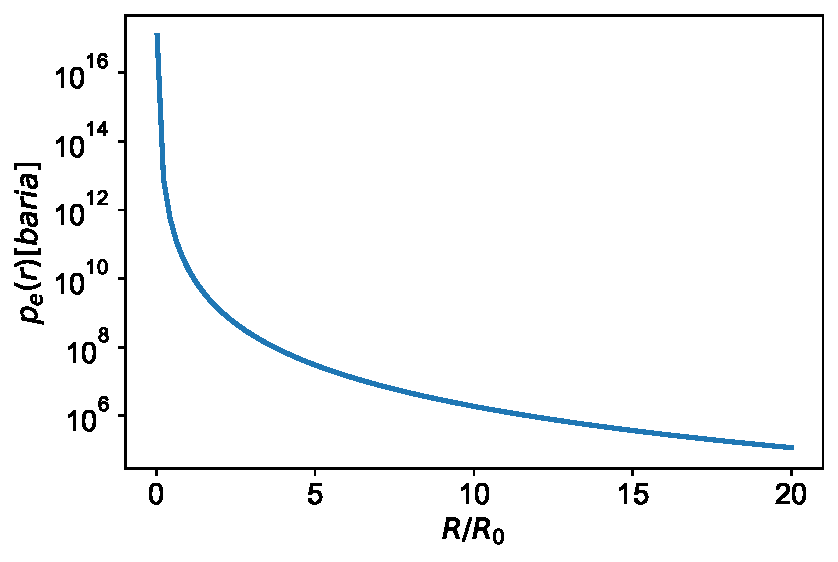
\includegraphics[clip=true,width=\columnwidth]{cap1_p_e_vs_R.pdf}
  \caption{\textcolor{blue}{Gráfico de la presión para ver su dependencia con $1/R^4$}}
   \label{fig:cap1_p_e_vs_R}
\end{figure}
\textcolor{red}{Discusión de la dependencia}

\ptitle{Presentación de la ecuación diferencial de evolución de $R(t)$}
\begin{itemize}
  \item A continuación se verá que la presión eléctrica produce que el bubston se expanda. Se parte de la ecuación de evolución de $R(t)$
  \item Esta es una aproximación de la ecuación de momento \textcolor{red}{Referencial el libro "The Acustic Bubble" de T.G.Leighton}
  \begin{equation}
    R \dot{u} + \frac{3}{2}u^2 = \frac{p_e}{\rho}
    \label{eq:bubston_ec_dif_R}
  \end{equation}
    \item donde $u = \dot{R} = dR/dt$ y se consideró que $p_e >> p_0$ presión hidrostática.
\end{itemize}



Dinámica de la burbuja para $R>R_0$
\begin{itemize}
  \item Dada la funcionalidad conocida de $p_e(R)$, lo único que queda es resolver la ecuación diferencial \ref{eq:bubston_ec_dif_R}.
  \item Esto se hizo numéricamente mediante el método Runge-Kutta-4.
  \item \textcolor{red}{Tengo que explicar en detalle cómo resolví numéricamente el problema?}
  \item \textcolor{blue}{Figura de R(t) marcando el límite en el que hay coalescencia}
  \item Esta evolución no vale indefinidamente, sino hasta que se produce la coalescencia de los bubstons del mismo cluster. Esto ocurre cuando $R(t) = R_1=l/2$ donde $l$ es la distancia entre los centros de los bubstons. Esta longitud se puede estimar como $l \approx 2a_i$
  \item \textcolor{red}{Revisar referencia y definir $a_i$}
  \item Numéricamente se obtuvo que el tiempo en el que ocurre este proceso $t_{coal}$ es del orden de \textcolor{red}{valor?}
\end{itemize}

\subsection{Evolución desde la formación del núcleo}

Armo el cuento desde la coalesciancia hasta llegar a los resultados importantes de radio máximo y el tiempo al que se da

\begin{itemize}
  \item Luego del tiempo de coalescencia se asume que todos los bubstons se fusionan para formar una burbuja grande, a partir de ahora denominada "núcleo".
  \item Condciones iniciales de la burbuja
  \item Calculo los distintos parámetros en función de las fórmulas presentadas
  \item 
  \item Se busca calcular la presión eléctrica en $R = R_{cl}$ a tiempo inicial. La presión eléctrica está dada por la ecuación (17) del Bunkin
  \[p_{e} = \frac{2}{3}\bar{n_e} T_e \frac{x}{3} \left [1 + \pi \left ( \frac{x-1}{x} \right )^2 \frac{e^2R_{cl}^2\bar{n_e}}{T_e}   \right ] \]
  donde $\bar{n_e} = 3.4 *10^{16} \, \mathrm{cm}^{-3}$ es la densidad media de electrones en el cluster, $T_e \approx 0.1 \, \mathrm{eV}$ es la temperatura de los electrones, $x \approx 17.9$ es un parámetro, $e$ es la carga eléctrica y $R_{cl}$ es el radio del cluster que a $t=0$ es $R_{cl} \approx 10^{-2} \, \mathrm{cm}$.  

  \item A partir de ahora puede dejar de valer el "régimen de autoconsistencia", por lo que la dependencia de $T(R)$ presentada en \textcolor{red}{referencia?} podría dejar de valer. En este sentido, se asume que los electrones del núcleo se encuentran a la misma temperatura correspondiente al instante anterior a la coalescencia, es decir, $T(R_1) \approx 0.1 eV$.



  \item Debido a que no se conoce el proceso por el cual los bubstons forman el núcleo, tampoco se puede asumir que la distribución de electrones $n_e(r)$ mantenga la funcionalidad de la expresión \textcolor{red}{referencia}. Consecuentemente, la expresión para la presión eléctrica también deja de valer. Aún más, la ecuación de evolución \ref{eq:bubston_ec_dif_R} deja de valer debido a que durante la dinámica del clúster podría ocurrir que la presión eléctrica sea comparable con la hidrostática externa. 

  \item Sin embargo, sí sepuede asumir $\dots$ \textcolor{red}{para continuar tengo que repasar las condiciones de la fórmula de Willis}
  \item \textcolor{red}{condiciones para la fórmula de Willis. Buscar bien y explicar por qué se plantea la igualdad de energías a tiempo inicial. No me queda claro por qué deja de valer la evolución que hicimos con la presión de electrones.}

  \item 
  \begin{equation}
    R \dot{u} + \frac{3}{2}u^2 = \frac{p_0}{\rho}
  \end{equation}


  \item La velocidad inicial está dada por 
  \item \textcolor{blue}{fórmula de la velocidad inicial en función de la energía}
  \item 
  \item Mientras que las condiciones iniciales son 
  \item Se obtuvo el radio máximo $\mathrm{R_{max}} = $ \textcolor{red}{valor?} cm a tiempo $\mathrm{t_{max}} = $ \textcolor{red}{valor?} s.
\end{itemize}






























\section*{Capítulo II: Evolución desde el radio máximo}

\subsection{Resumen del capítulo}

\ptitle{Descripción general de los fenómenos}
\begin{itemize}
  \item El objetivo es calcular la evolución de una burbuja de radio inicial $R_{max}$ \textcolor{red}{tiene que tener el mismo nombre que el cap anterior} hasta el estado de compresión máxima.
  \item En el capítulo anterior solo se tuvieron en cuenta las fuerzas hidrostáticas y eléctricas. En este capítulo se consideran no se considerarán las fuerzas eléctricas.
  \item Se considerarán una gran variedad de efectos físicos que se demostraron son importantes en la evolución de la burbuja \textcolor{red}{Referencia a Gabriela}
  \item Estos son la compresibilidad y viscosidad del medio líquido que rode a la burbuja, la transferencia de calor, la transferencia de masa debido a condensación y evaporación del vapor, la difusión de las partículas de vapor y la variación del número de partículas de distintas especies debido a reacciones químicas.
  \item El objetivo es calcular la evolución del radio $R(t)$ de la burbuja
\end{itemize}

\ptitle{Ecuación diferencial para $R(t)$}
\begin{itemize}
  \item La evolución del radio $R(t)$ de la burbuja está dada por la ecuación de Rayleigh y Plasset generalizada \textcolor{red}{Referencia al Yasui. No sé a cuál de todos. Fijarme que el paper tenga la misma ecuación}
  \begin{equation}
    \left ( 1 - \frac{\dot{R}}{c_L}  + \frac{\dot{m}}{c_L \rho_{L,i}}   \right ) R \ddot{R} + \frac{3}{2} \dot{R}^2 \left (  1 - \frac{\dot{R}}{3 c_L} + \frac{2 \dot{m}}{3 c_L \rho_{L,i}}  \right ) = \frac{1}{\rho_{L,i}} \left ( 1 + \frac{\dot{R}}{c_L} \right )  \left ( p_B - p_\infty \right ) + \frac{\ddot{m} R}{\rho_{L,i}} \left ( 1 - \frac{\dot{R}}{c_L} + \frac{\dot{m}}{c_L \rho_{L,i}} \right ) + \frac{\dot{m}}{\rho_{L,i}} \left ( \dot{R} - \frac{\dot{m}}{2 \rho_{L,i}} + \frac{\dot{m}\dot{R}}{2 c_L \rho_{L,i}}  \right ) + \frac{R}{c_L \rho_{L, \infty}} \frac{d p_B}{dt}
    \label{eq:cap2_R_ecdif}
  \end{equation}
  donde $c_L$ es la velocidad del líquido en el infinito, $\dot{m}$ es el flujo neto de evaporación por unidad de área y unidad de tiempo,$\rho_{L,i}$ es la densidad del líquido en la superficie de la burbuja, $\rho_{L, \infty}$ es la densidad del líquido en el infinito, $p_B(t)$ es la presión del líquido sobre la superficie externa de la burbuja y $p_\infty$ es la presión ambiente en el infinito.
  \textcolor{blue}{Presentar ecuación, de dónde se obtuvo, qué es cada factor y de dónde se sacan los valores, son los mismos para deuterio e hidrógeno?}
\end{itemize}


\ptitle{¿Dónde se considerará cada fenómeno?}
\begin{itemize}
  \item ¿Dónde serán tenidos en cuenta los fenómenos físicos comentados anteriormente?
  \item La compresibilidad y viscodidad del medio líquido fueron tenidas en cuenta en la ecuación de $R(t)$
  \item Para calcular $\dot{m}$ es necesario considerar la evaporación y condensación en las paredes de la burbuja, así como la transferencia de calor.
  \item Para calcular $p_B$ se necesita una ecuación de estado del gas interno
  \item Para calcular $\frac{dp_B}{dt}$ se necesita conocer cómo varía el número de partículas de cada especie dentro de la burbuja a través de reacciones químicas y, para el caso particular de gases condensables, se necesitan considerar difusión. Además, se ncesita conocer cómo varía la temperatura de la burbuja, necesitando una ecuación para la conservación de la energía
\end{itemize}

\ptitle{¿Qué fenómenos se implementaron en este trabajo?}
\begin{itemize}
  \item Comentar que en este trabajo se logró implementar el código de reacciones y de condensación/evaporación.
  \item Comentar qué modelo se considera para la presión de los gases dentro de la burbuja y qué modelo para la energía
  \item Comentar que se trata de un problema del tipo stiff y deberá ser trabajado con cuidado. No definir problemas stiff, eso conviene hacerlo en otra sección.
\end{itemize}

\ptitle{Descripción física del problema}
\begin{itemize}
  \item \textcolor{red}{Lo que escribo acá estaría bueno mencionarlo arriba en algún lugar}
  \item La burbuja consta de un gas interno que se asume está a una temperatura uniforma $T$ salvo por una capa superficial cerca de la pared de la burbuja. El gas en la sección interior de la capa se encuentra a temperatura $T_{B,i}$, mientras que el líquido en la sección exterior se encuentra a temperatura $T_{L,i}$.
  \item Esto está propuesto por resultados teóricos de la referencia [22] en el paper de Yasui 1997.
  \item El salto de temperatura en la interfase se puede demostrar mediante teoría cinética de gases \textcolor{red}{Esto está referenciado en Yasui 1997 y en la tesis de Gabriela}
  \item \textcolor{blue}{Podría agregarse una imagen representativa para mayor claridad}
\end{itemize}


\subsection{Fenómenos físicos}

\subsubsection{Condensación y Evaporación}

\begin{itemize}
  \item Tengo que repasar la tesis de Gabriela y el paper de Yasui para comenzar a escribir esto
  \item Sí se podría hacer mención a las ecuaciones para calcular la conducción de calor.
\end{itemize}

\ptitle{Definición de $\dot{m}$}
\begin{itemize}
  \item El flujo neto de evaporación por unidad de área y tiempo $\dot{m}$ es la diferencia entre el flujo de evaporación $\dot{m}_{eva}$ y el de condensación $\dot{m}_{cond}$, es decir,
  \item \[\dot{m} = \dot{m}_{eva} - \dot{m}_{cond} \]
  \item Estos flujos están dados por
  \[\dot{m}_{eva} = \frac{\alpha_M}{\sqrt{2 \pi R_v}} \frac{p_v^*}{\sqrt{T_{L,i}}} \]
  \[\dot{m}_{cond} = \frac{\alpha_M}{\sqrt{2 \pi R_v}} \frac{\Gamma p_v}{\sqrt{T_{B,i}}}  \]
  \textcolor{red}{Esta fórmula no es la misma que está en Yasui 1997 pero sí es la misma que en el Fujikawa 1980 al que Yasui tmb cita. La diferencia está en un factor $10^3 N_A / M_{H_2O}$. ¿A cuál le hago caso?}
  \item donde $\alpha_M$ es el coeficiente de acomodación para los procesos de evaporación o condensación, $R_v$ es la constante de los gases ideales para el vapor definido como
  \item \textcolor{red}{definición}
  \item , $p_v$ es la presión parcial correspondiente al vapor
  \item \[p_v = \frac{n_v}{n_{tot}} p_{tot} \]
  \item con $n_v$ número de partículas de vapor, $n_{tot}$ número total de partículas y $p_{tot}$ presión total dentro de la burbuja. Además, $p_v^*$ es la presión de vapor saturado a la temperatura del líquido en la interfase $T_{L,i}$ y $T_{B,i}$ es la temperatura del gas en la interfase.
  \item El factor de corrección $\Gamma$ está dado por la siguiente expresión
  \item \[\Gamma = e^{-\Omega^2} - \Omega \sqrt{\pi} \left ( 1 - \frac{2}{\sqrt{\pi}} \int_0^{\Omega} e^{-x^2} dx \right ) \]
  \item con \[\Omega = \frac{\dot{m}}{p_v} \sqrt{\frac{R_v T_{B,i}}{2}}\]
  \item \textcolor{red}{En esta última expresión Gabriela copia al Yasui el cual dice que en $\Omega$ aparece $T$ la temperatura en el interior de la burbuja. Sin embargo, en el Fujikawa 1980 aparece $T_{B,i}$ la temperatura en la interfase. ¿A cuál le hago caso?}
\end{itemize}

\subsubsection{Presión y ecuación de estado}

\ptitle{Definición de $p_B$ presión del líquido sobre la superficie externa de la burbuja}
\begin{itemize}
  \item La presión del líquido sobre la superficie externa de la burbuja $p_B$ presente en \ref{eq:cap2_R_ecdif} está dada por la expresión
  \item \[p_B(t) = p_g(t) -\frac{2 \sigma}{R} - \frac{4 \mu}{R} \left ( \dot{R} - \frac{\dot{m}}{\rho_{L,i}} \right ) - \dot{m}^2 \left ( \frac{1}{\rho_{L,i}} - \frac{1}{\rho_g} \right ) \]
  \item donde $p_g(t)$ es la presión en el interior de la burbuja, $\sigma$, la tensión superficial, $\mu$, la viscosidad del líquido y $\rho_g$, la densidad total en el interior de la burbuja.
\end{itemize}

\ptitle{Definición de la presión en el interior de la burbuja $p_g$. Ec de estado de Van der Waals.}
\begin{itemize}
  \item La presión en el interior de la burbuja $p_g$ se modeló mediante la ecuación de Van der Waals \textcolor{red}{referencia?}
  \item , válida para un range amplio de temperaturas \textcolor{red}{y presiones?}
  \item \[p_g(t) = \frac{R_g T}{\nu - b} - \frac{a}{\nu^2}\]
  \item donde $R_g$ es la constante universal de los gases, $T$ es la temperatura de la mezcla en el interior de la burbuja \textcolor{red}{Esto ya lo dije antes}, $\nu$ es el volumen molar de la mezcla de gases en el interior de la burbuja \textcolor{red}{Buscar qué es esto exactamente. Está referenciado en Yasui 1996} y $a$ y $b$ son las constantes de Van der Waals de la mezcla. Estas constantes están dadas por
  \item \[a = a_{H_2O}, b = b_{H_2O} \]
  \item \textcolor{red}{La fórmula anterior no es la de Gabriela}
  \item \textcolor{red}{Uso el modelo de Van der Waals usando combinaciones lineales de las ctes. Esto se justifica en Beattie 1930. No se hace exactamente una combinación lineal de las constantes pesadas por las fracciones molares, es algo un poco más complicado. En Beattie 1930 también se mencionan otros modelos "actuales" que sirven para mezclas de gases. En Yasui 1997 se usa la misma fórmula que Gabriela considerando Argón y no se toman más gases bajo el justificativo de que "el efecto de los productos químicos en las ctes de van der Waals se desprecia debido a que la cantidad de productos químicos es pequeña. Toegel 2003 usa otro modelo similar al de Van Der Waals}
  \item \textcolor{red}{Tengo que buscar cómo es esta expresión porque hay una gran variedad de gases}
  \item Dichas constantes cambian en el tiempo debido a la variación en la cantidad de moléculas de cada especie.
\end{itemize}

\subsubsection{Transferencia de calor}

\ptitle{Diferencia entre $T_{B,i}$ y  $T_{L,i}$}
\begin{itemize}
  \item Mediante teoría cinética de gases se puede demostrar que el salto de temperatura en la capa superficial de la burbuja es
  \item \[T_{B,i} - T_{L,i} = \Delta T = -\frac{1}{2 k n'} \sqrt{\frac{\pi \bar{m}}{2 k T_{B,i}}} \frac{2 - a' \alpha_E}{\alpha_E} q''|_{r = R} \]
  \item donde $k$ es la constante de Boltzmann, $n'$ es la densidad de partículas totales (gas y vapor), $\bar{m}$ es la masa media de una molécula \textcolor{red}{No es clara esta def}, $a' = 0.827$ es una constante que depende del gas \textcolor{red}{verficar referencia} y $q''|_{r = R}/\kappa$ es el gradiente de temperatura del lado interno de la superficie de la burbuja, con $\kappa$ conductividad térmica de la mezcla de gases.
\end{itemize}

\ptitle{Expresión de $q''$. Modelo de Toegel}
\begin{itemize}
  \item \textcolor{red}{La expresión de la tesis de Gabriela según el modelo de Toegel (2.2.9.2.1) es distinta de la del modelo de Toegel en sí (Toegel 2000)}

\end{itemize}

\subsubsection{Reacciones químicas}


\ptitle{Presentación de $\dot{N}_i^{chemical}$}
\begin{itemize}
  \item Las reacciones químicas dentro de la burbuja son de no equilibrio \textcolor{red}{Referencia al libro de Yasui} y es necesario emplear un modelo de cinética química
  \item Ocurren cuando las temperaturas en el interior de la burbuja son elevadas
  \item En este trabajo se consideró sólo la presencia inicial de moléculas de $\mathrm{H_2O}$, $\mathrm{O_2}$ y $\mathrm{H_2}$, lo cual da lugar a \textcolor{red}{8} reacciones
  \item Estas se encuentran tabuladas en la tabla \textcolor{red}{Referencia a la tabla}
  \item El cambio total del número de partículas de la especie $i$ debido a todas las reacciones químicas en las que se encuentra involucrada está dado por
  \[\dot{N}_i^{chemical} = V \sum_j{\alpha_{i,j} r_j} \]
  \item \textcolor{red}{En la fórmula de Gabriela también está el factor "Na" dividiendo que creo que es el nro de Avogadro. Tengo que verificar esto en el código de Gabriela}
  \item \textcolor{red}{Referenciar a Gabriela y a Toegel 2003.}
  \item donde $V = 4 \pi R^3 /3$ es el volumen de la burbuja, $alpha_{i,j}$ el coeficiente estequiométrico de la especie $i$ en la reacción $j$ y $r_j$ es la velocidad de reacción de la reacción $j$.
\end{itemize}

\ptitle{Velocidad de reacción}
\begin{itemize}
  \item La velocidad de reacción $r_j$ está dada por la diferencia entre las reacciones por adelante ('forward') y por atraso ('backward')
  \[r_{j} = r_{f,j} - r_{b,j} \]
  \item donde $r_{f,j}$ y $r_{b,j}$ están descriptas por la ecuación de Arrhenius modificada \textcolor{red}{referencia. En el Toegel 2003 hay una} y pueden tomar distintas expresiones dependiendo de cuántos cuerpos hay involucrados en la reacción. 
\end{itemize}


\ptitle{Velocidad de reacción para $A + B \leftrightarrow  C + D$}
\begin{itemize}
  \item Para un proceso del tipo $A + B \leftrightarrow  C + D$ se tiene en el límite de baja densidad \textcolor{red}{ref Toegel 2003}
  \[
  \left\{\begin{matrix}
   r_{f,j} = k_{f,j} n_A n_B T^{c_{f,j}} \exp{(-\frac{E_{f,j}}{k T})} \\
   r_{b,j} = k_{b,j} n_C n_D T^{c_{b,j}} \exp{(-\frac{E_{b,j}}{k T})}
   \end{matrix}\right.
   \]
   donde $n_i$ es la concentración de la especie $i$
\end{itemize}

\ptitle{Velocidad de reacción para $M + A + B \leftrightarrow  M + C$}
\begin{itemize}
   \item Mientras que para un proceso del tipo $M + A + B \leftrightarrow  M + C$ se tiene 
   \[
   \left\{\begin{matrix}
    r_{f,j} = \beta^{t_j} k_{f,j} n_{tot} n_A n_B T^{c_{f,j}} \exp{(-\frac{E_{f,j}}{k T})} \\
    r_{b,j} = k_{b,j} n_{tot} n_C T^{c_{b,j}} \exp{(-\frac{E_{b,j}}{k T})}
    \end{matrix}\right.
   \]
   donde
   \[\beta  = \frac{\exp{ \left (  \frac{n_{tot} B}{1 - n_{tot} B}  \right )   }  }{1 - n_{tot} B} \]

\end{itemize}


\begin{table}[]
  \centering
  \begin{tabular}{llllllllll}
    \hline
    \multicolumn{1}{|l|}{j} &
    \multicolumn{1}{l|}{Reacción} &
    \multicolumn{1}{l|}{$t_j$} &
    \multicolumn{1}{l|}{$k_{f,j}$} &
    \multicolumn{1}{l|}{$c_{f,j}$} &
    \multicolumn{1}{l|}{$E_{f,j}/k$} &
    \multicolumn{1}{l|}{$k_{b,j}$} &
    \multicolumn{1}{l|}{$c_{b,j}$} &
    \multicolumn{1}{l|}{$E_{b,j}/k$} &
    \multicolumn{1}{l|}{$\Delta E_j$} \\ \hline
  1  & $\mathrm{O + O + M \leftrightarrow O_2 + M} $ &1      &1.2e17           &-1  &0  &3.16e19  &-1.3 &59893  & 498 \\
  2  & $\mathrm{O + H + M  \leftrightarrow OH + M} $ &1      &5e17           &-1  &0  &3.54e17  &-0.9  &51217 & 428\\
  3  & $\mathrm{O + H_2  \leftrightarrow H + OH} $ &0       &3.87e4           &2.7  &3150  &1.79e4  &2.7  &2200  &-8  \\
  4  & $\mathrm{H + O_2  \leftrightarrow O + OH} $ &0       &2.65e16           &-0.7  &8576  &9e13  &-0.3  &-83  &-70  \\
  5  & $\mathrm{H + H + M  \leftrightarrow H_2 + M} $ &1       &1e18           & -1  &0  &7.46e17  &-0.8  &52177 &436 \\
  6  & $\mathrm{H + OH + M  \leftrightarrow H_2O + M} $ &1       &2.2e22           &-2  &0  &3.67e23  &-2  &59980  &498  \\
  7  & $\mathrm{ OH + H_2  \leftrightarrow H + H_2O} $ &0       &2.16e8           &1.5  &1726  &5.2e9  &1.3  &9529  &62  \\
  8  & $\mathrm{ OH + OH \leftrightarrow O + H_2O} $ &0       &3.57e4           &2.4  &1062  &1.74e6  &2.2  &7693  &70 \\
  9  & $\mathrm{HO_2 + HO_2 \leftrightarrow H_2O_2 + O_2}$ & 0      &3.0e12           &0  &-700  &4.53e14  &-0.39  & -19700 & \textcolor{red}{??} \\
  10  & $\mathrm{H_2O_2 + M \leftrightarrow OH + OH + M}$ & 1      &1.2e17           &0  &-22900  &9.0e5  &0.9  & 3050 & \textcolor{red}{??} \\
  11  & $\mathrm{H_2O_2 + H \leftrightarrow H_2O + OH}$ & 0      &3.2e14           &0  &-4510  &1.14e9  &1.36  & -38180 & \textcolor{red}{??} \\
  12  & $\mathrm{H_2O_2 + H \leftrightarrow H_2 + HO_2}$ & 0      &4.82e13           &0  &-4000  &1.41e11  &0.66  & -12320  & \textcolor{red}{??} \\
  13  & $\mathrm{H_2O_2 + O \leftrightarrow OH + HO_2}$ & 0      &9.55e6           &2  &-2000  &4.62e3  &2.75  & -9277 & \textcolor{red}{??} \\
  14  & $\mathrm{H_2O_2 + OH \leftrightarrow H_2O + HO_2}$ & 0      &1.0e13           &0  &-900  &2.8e13  &0  & -16500 & \textcolor{red}{??} \\ \hline
\end{tabular}
\end{table}







Gabriela obtuvo el modelo de reacciones qcas del paper de Yasui 1997. \textcolor{red}{Podría verificar si no hay un mejor modelo}.
Yasui escribió un libro sobre burbujas. Quicás sea útil leerlo. Mi principal foco estaría en el capítulo 2. Se desarrollan no solo las reacciones químicas sino también los demás fenómenos.

Toegel Phase diagrams for sonoluminescing bubbles: A comparison between experiment and theory. En este se desarrolla el modelo hidrondinámico de la burbuja, junto tmb a modelos de transferencia de calor. En cuanto a las reacciones químicas en particular, el modelo no es exactamente el de la ecuación de Arrhenius, sino de la "ley de Arrhenius modificada". En teoría esto se explica en mayor detalle en el libro "Gas-Phase Combustion Chemistry" de W. C. Gardiner pero no me puse a buscarlo



\begin{itemize}
  \item Releer la parte de reacciones químicas de la tesis de Gabriela y el paper de Yasui al que se hace referencia. Esta sección intenta resumir eso.
  \item \textcolor{red}{DUDA: en el código de Gabriela, n es nro de partículas o concentración? En la tesis es concentración}
  \item \textcolor{red}{Vale la pena agregar acá la contribución de las reacciones químicas a la conservación de la energía?}
\end{itemize}





\subsection{Método numérico}

\begin{itemize}
  \item Mencionar que es un problema del tipo stiff. Explicar brevente de qué se trata esto
  \item Historia de cómo el código pasó de ejecutar en días (el mío) o minutos (el de Gabriela) a segundos (el mío):
  \item Comentar que ya se contaba con un código en C++ programado en Borland por Gabriela (y en qué año), pero que resolvía el sistema de ecuaciones diferenciales usando Runge-Kutta Ferhber \textcolor{red}{corroborar cómo se escribía}. Comentar qué complicaciones tenía y que se progrmó toro código en C++
  \item Se usó el cluster.
  \item Se optó por python. Se usó la librería scipy. Nuevamente el código era muy lento con RK45 pero con el método de Radau todo mejoró. \textcolor{red}{Explico esto?}
\end{itemize}















































\section*{Conclusiones}
\begin{enumerate}
  \item Se calculó numéricamente el radio máximo de la burbuja, obteniendo un valor 10 veces mayor a los resultados experimentales (y teóricos del Bunkin)
  \item Se calculó numéricamente el tiempo al que la burbuja alcanza el radio máximo, obteniendo un valor 10 veces mayor a los resultados experimentales (y teóricos del Bunkin)
  \item Ídem para la energía, salvo por un factor 600
  \item Se encontró que el problema es de naturaleza stiff, lo cual permitió elegir un mejor método numérico que el que se venía usando. Esto permitió disminuir enormemente el tiempo de cómputo
  \item Se logró calcular la evolución de un único bubston, obteniendo los mismos resultados que el paper de Bunkin
  \item Se logró implementar un módulo de reacciones, de conducción del calor y de condensación y evaporación.
  \item Se pudo usar el cluster de MECOM para agilizar las cuentas del código en C++, aunque luego se decidió trabajar en python
  \item Se lograron reproducir las  cuentas más importantes del Bunkin con Mathematica



\end{enumerate}




\bibliography{Chehade_tesis.bib}

\end{document}





